\begin{figure}
	\centering
	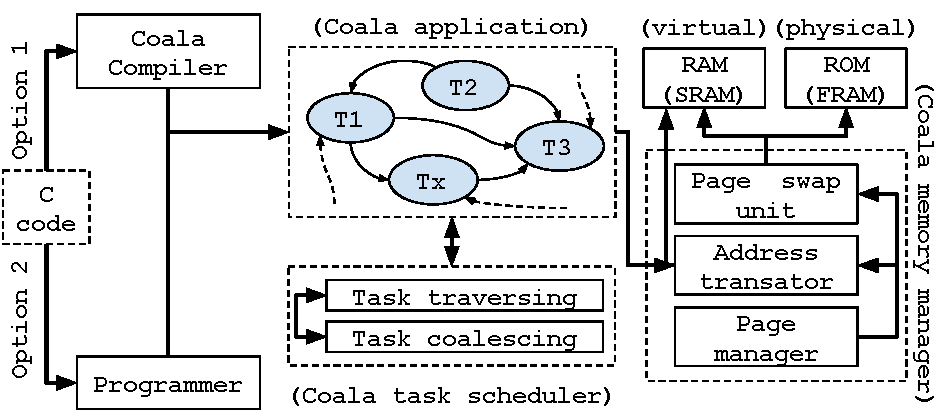
\includegraphics[width=\columnwidth]{figures/viper_block_diagram.pdf}
	\caption{\sys top-level view.}
	\label{fig:system_overview}
\end{figure}

\sys as a whole is characterized by the following features:

\begin{itemize}
	\item \textbf{Compiler-supported automatic task generator}: details will be provided in Section~\ref{sec:compiler}
	\item \textbf{Memory virtualization}: details will be provided in Section~\ref{sec:memory_virtulaization}
	\item \textbf{Task coalescing}: details will be provided in Section~\ref{sec:task_coalescing}
\end{itemize}

A complete logical structure of \sys is given in Figure~\ref{fig:system_overview}. Before describing each feature of \sys in detail we need to introduce a programming and semantics/execution model.

\begin{figure}
	\centering
	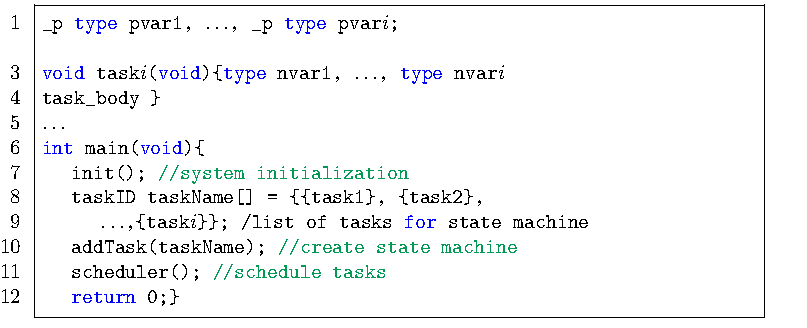
\includegraphics[width=\columnwidth]{figures/taskification_example}
	\caption{\sys API.}
	\label{fig:system_overview}
\end{figure}


\subsection{Programming Model}
\label{sec:overview_programming_model}

\begin{table}
	\centering
	\footnotesize
	\begin{tabular}{|c|c|}
		\hline
		Keyword & Description\\
		\hline\hline
		\texttt{RP} & Read-protected variable\\
		\texttt{WP} & Write-protected variable\\
		\texttt{\_\_task\_\_ foo(){...}} & Task declaration\\
		\texttt{addTask()} & Build internal data structure for executor \\
		\texttt{run\_tasks()} & Task executor \\ %scheduler
		\texttt{next\_task()} & Transition to a new task\\
		%\texttt{PageFault()} & --- \\
		%\texttt{P()} & ---\\
		\hline
	\end{tabular}
\caption{Summary of \sys syntax: top---user-specific variables}
\label{tab:viper_syntax}
\end{table}

\subsection{Semantics and Execution Model}
\label{sec:overview_semantics}

